\chapter{Analisis dan Perancangan}

\section{Analisis Masalah}

Tujuan dari penelitian ini adalah membuat sebuah sistem permainan musik ekspresif alat musik gesek yang mampu menghasilkan suara musik ekspresif hanya dari masukan partitur saja. Untuk itu, akan dianalisis masalah-masalah yang ada dalam membangun sistem tersebut dan akan dirancang solusinya.

Subsistem yang telah ada untuk alat gesek dari penelitian-penelitian sebelumnya tidak dapat digabungkan secara langsung. Hal ini karena keluaran dari sistem perencana gestur dan perencana ekspresi tidak sesuai dengan masukan sistem sintesis. Karena itu, dibutuhkan suatu sistem di mana perencana gestur dan perencana ekspresi yang terintegrasi atau memiliki keluaran sesuai dengan sistem sintesis.

Terdapat dua alternatif pilihan untuk mencapai hal ini:

\begin{enumerate}
	\item membuat sistem di mana perencana gestur dan perencana ekspresi terpisah, dengan keluaran perantara berupa representasi rencana gestur dan rencana ekspresi
	\item membuat sistem yang langsung membangkitkan suara ekspresif dari partitur
\end{enumerate}

Pilihan pertama, yaitu membuat sistem terpisah, memiliki kendala dalam hal representasi rencana gestur dan rencana ekspresi dan anotasi. Meski representasi dapat dirancang dengan tangan, pencarian representasi yang tepat membutuhkan usaha yang sangat besar. Selain itu, kesesuaian representasi tersebut sulit divalidasi terhadap data. Adapun anotasi manual rencana gestur dan rencana ekspresi, berdasarkan penelitian-penelitian sebelumnya yang telah disebutkan di Bab 2, memiliki peluang kesalahan yang sangat besar.

Karena itu, akan dibuat sistem yang langsung membangkitkan suara ekspresif dari partitur. Terdapat banyak pendekatan membangkitkan suara dari partitur. Khusus untuk membangkitkan suara yang ekspresif dari partitur tanpa adanya rencana gestur ataupun rencana ekspresi, terdapat dua alternatif:

\begin{enumerate}
	\item membangkitkan waveform secara langsung
	\item membangkitkan parameter vocoder, yang kemudian digunakan oleh vocoder untuk mensintesis suara
\end{enumerate}

Akan digunakan digunakan teknik vocoder karena cara membangkitkan waveform secara langsung membutuhkan waktu yang lama (tidak realtime). Untuk teknik vocoder ini, terdapat beberapa perbedaan masalah dengan penelitian sebelumnya\parencite{bonada2017singing}. Perbedaan masalah yang terjadi terdapat pada data input untuk sintesis, data latih, timing, dan konteks.

Perbedaan masalah untuk data input sintesis terkait dengan timbre. Dalam pembangkitan suara alat musik gesek, timbre ditentukan oleh konteks. Hal ini berbeda dengan penelitian sebelumnya, di mana timbre ditentukan dari rangkaian fonem yang terdapat dalam data input.

Perbedaan masalah terkait dengan data latih terdapat pada pewaktuan. Dalam penelitian ini, pewaktuan tidak terdapat pada data input.

Timing not dalam alat musik gesek memiliki karakteristik yang berbeda dengan suara nyanyian. Dalam sistem baseline untuk suara nyanyian, timing not menyesuaikan dengan timing fonetik. Dalam sistem ini, tidak ada fonetik yang eksplisit yang dapat diikuti oleh timing not.

Perbedaan masalah terkait konteks yaitu pada medan reseptif dari jaringan syaraf tiruan pada baseline. Baseline yang digunakan memiliki medan reseptif 100ms. Untuk membangkitkan suara ekspresif, dibutuhkan konteks global dan konteks lokal dari not. Selain itu, konteks juga dibutuhkan dalam timbre.

\section{Rancangan Umum Sistem}

Untuk mengatasi masalah-masalah yang telah disebutkan, akan digunakan teknik neural parametrik serupa dengan baseline\parencite{bonada2017singing} dengan modifikasi. Modifikasi pertama yang diajukan adalah modifikasi pada arsitektur umum sistem. Modifikasi kedua yang diajukan dilakukan kepada arsitektur jaringan syaraf tiruan.

Arsitektur sistem yang diajukan terlihat pada gambar \ref{fig-system-overview}. Dalam sistem ini, tidak ada masukan timing fonetik untuk pelatihan. Partitur yang menjadi masukan pun tidak memiliki deskripsi fonem dan lirik. Model timing fonetik diganti menjadi model timing. Dalam sistem ini, ada komponen tambahan yaitu alignment dan analisis timing.

Dalam sistem ini, timing tidak diberikan dari data masukan. Karenanya, timing harus mampu diinferensi dari masukan partitur dan audio saja. Untuk inferensi timing dari audio dan partitur, digunakan teknik alignment menggunakan masukan partitur dan hasil analisis vocoder dari audio. Hasil analisis vocoder yang digunakan adalah frekuensi fundamental dan kesunyian.

Berbeda dengan sistem baseline, model timbre yang diajukan dalam sistem ini harus mampu menentukan timbre dari konteks partitur. Karenanya, model timbre dalam pelatihan menerima masukan partitur, timing, dan dilatih untuk memprediksi data analisis vocoder. Parameter analisis vocoder yang diprediksi oleh model timbre adalah spectral envelope dan komponen aperiodic.

Model timing dalam sistem ini dilatih menggunakan partitur dan hasil analisis timing. Dengan demikian, diharapkan model timing dapat memprediksi timing dari not dalam partitur.

Model pitch dalam sistem ini dilatih untuk menghasilkan F0. Masukan model ini adalah partitur dan timing. Dalam pelatihan, masukan partitur diambil dari data latih, timing diambil dari hasil alignment dan analisis timing, dan parameter vocoder diambil dari hasil analisis vocoder terhadap audio.

\begin{figure}[h]
    \centering
    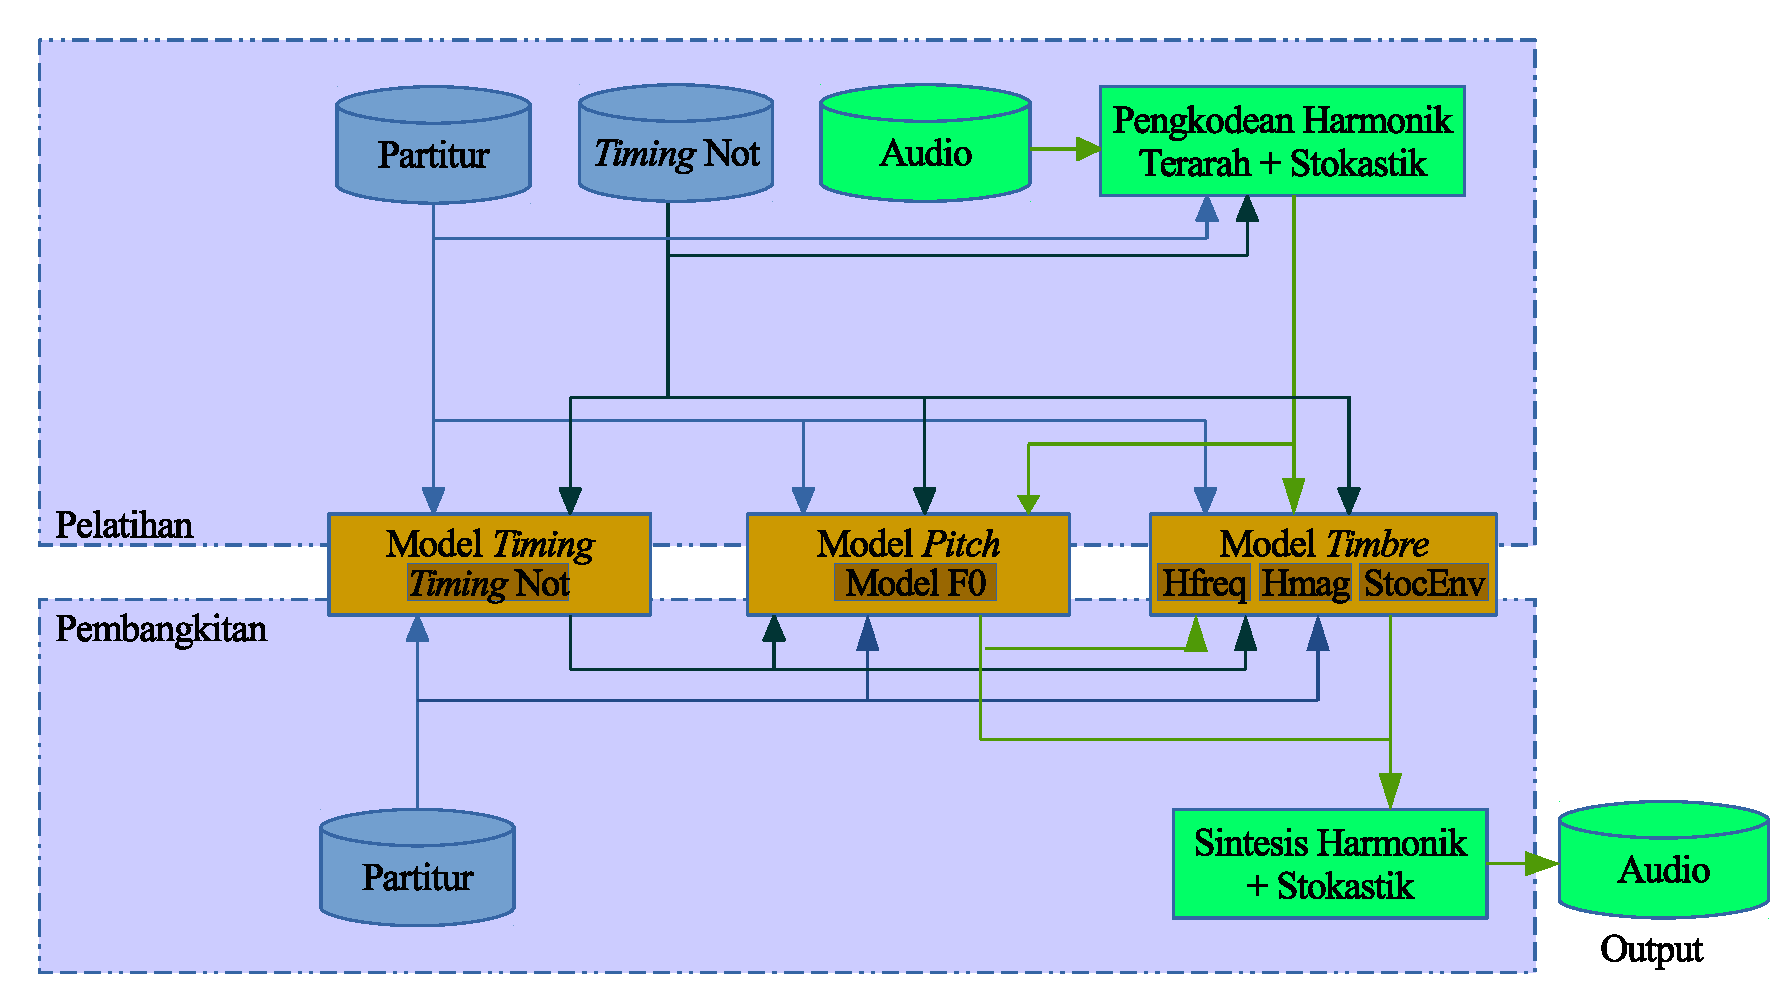
\includegraphics[width=0.8\textwidth]{resources/system-overview.eps}
    \caption{Arsitektur sistem permainan musik ekspresif alat musik gesek yang diajukan}\label{fig-system-overview}
\end{figure}

Pada tahap pembangkitan, sistem ini mampu menerima partitur dan menghasilkan audio. Keluaran perantara yang dihasilkan adalah parameter vocoder, yang kemudian digunakan oleh vocoder untuk menghasilkan audio.

Hal pertama yang dilakukan dalam tahap pembangkitan adalah prediksi timing not. Setelah itu, partitur dan timing not digunakan untuk memprediksi pitch an timbre, dengan model yang sesuai. Parameter pitch -frekuensi fundamental- dan parameter timbre -spectral envelope dan aperiodisitas- digunakan untuk sintesis vocoder.

Tiap model dari model-model ini adalah model regresi. Model regresi yang digunakan adalah jaringan syaraf tiruan konvolusional terdilasi dengan elemen rekuren. Masukan dari jaringan syaraf tiruan ini terdiri dari masukan rekuren -output pada waktu sebelumnya- dan masukan kontrol.

Masukan kontrol jaringan syaraf tiruan ini berasal dari tahap partitur dan dari timing. Untuk model timing, masukan kontrol hanya berasal dari partitur. Untuk model pitch dan model timbre, masukan kontrol berasal dari partitur dan berasal dari timing.

Masukan dari partitur dapat menunjukkan kondisi sesaat dan konteks. Kondisi sesaat berupa pitch asli, panjang not, dan waktu dalam not. Kondisi konteks dapat berupa not sebelum dan sesudah, interval, ataupun kondisi-kondisi lainnya hasil analisis karya. Namun, kakas analisis karya mungkin tidak akan digunakan karena riset terkait analisis karya menggunakan komputer masih minim.

\begin{figure}[h]
    \centering
    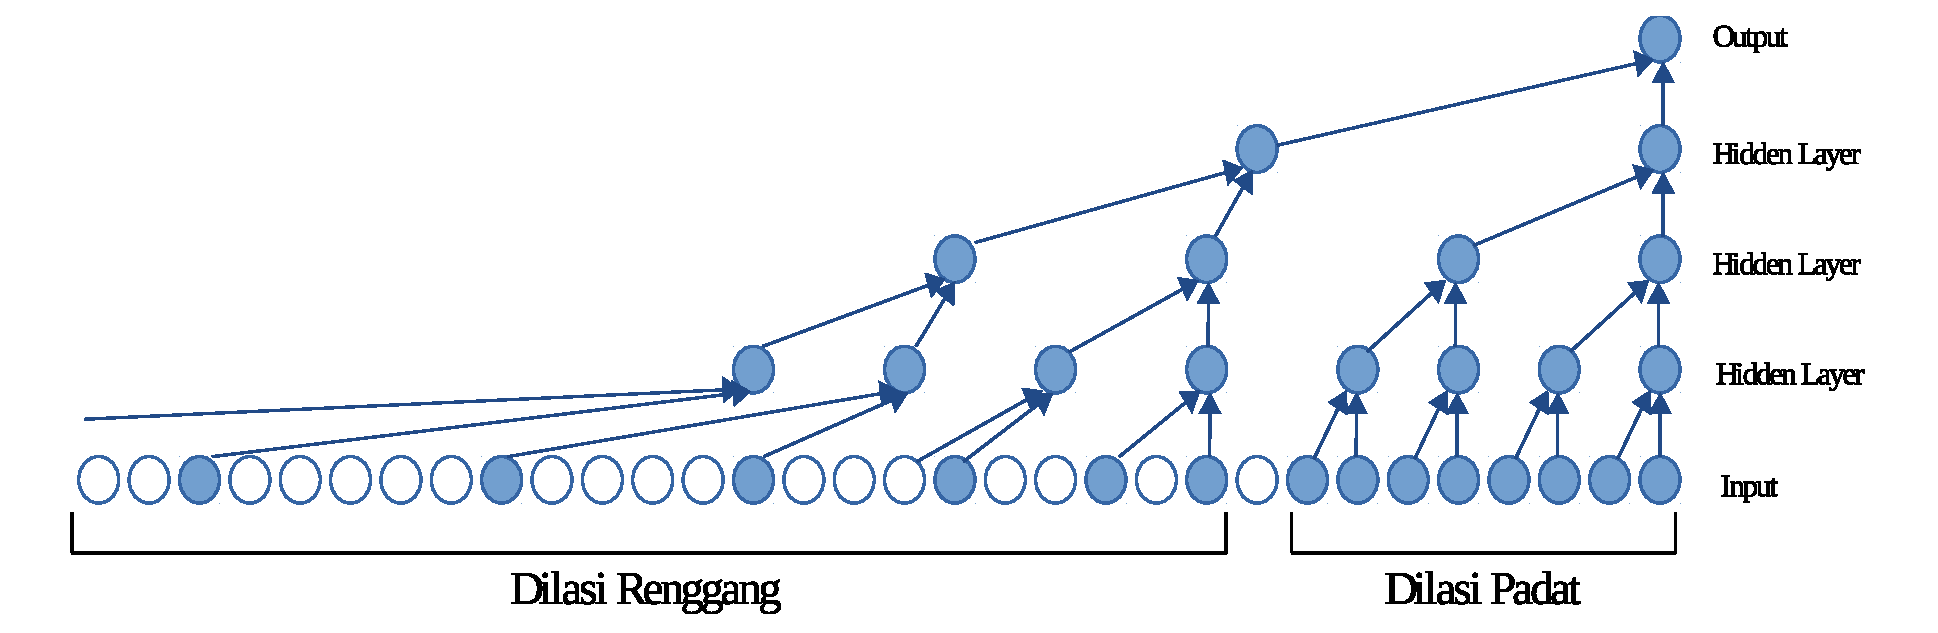
\includegraphics[width=0.8\textwidth]{resources/sparse-dense-dilated-cnn.eps}
    \caption{Arsitektur jaringan syaraf tiruan konvolusional dengan dilasi jarang-padat}\label{fig-sparsedilated-cnn}
\end{figure}

Untuk mengatasi masalah medan reseptif dari model baseline, diajukan dilasi jarang-padat. Arsitektur jaringan syaraf tiruan dengan modifikasi ini terlihat pada gambar \ref{fig-sparsedilated-cnn}. Untuk simpul-simpul masukan yang dekat dengan frame yang sedang dibangkitkan, digunakan faktor dilasi sedemikian hingga semua node terlingkupi. Untuk simpul-simpul masukan yang jauh dari frame yang sedang dibangkitkan, digunakan faktor dilasi yang lebih besar. Dengan demikian, medan reseptif dapat ditingkatkan tanpa menambah jumlah simpul tersembunyi dan ukuran vektor bobot yang diestimasi.

Pada bagian dengan dilasi jarang, ada simpul-simpul yang dilewat. Dalam permasalahan suara alat musik gesek, hal ini tidak menjadi masalah. Karakteristik suara yang menjadi masukan rekuren banyak redundan. Adapun masukan kontrol untuk simpul-simpul yang berdekatan akan sama karena satu not dapat menjadi banyak frame di mana tiap frame menjadi simpul masukan.

Untuk melatih sistem ini, dibutuhkan data latih berupa partitur dan rekaman audio. Data yang dibutuhkan adalah data berpasangan. Detil pengumpulan data latih ini dijelaskan dalam subbab selanjutnya.

\section{Pengumpulan Data}

Data yang dibutuhkan berupa data latih dan data uji. Dalam pengumpulan, data akan dihimpun menjadi satu kumpulan data. Kumpulan data tersebut akan dipisahkan menjadi data latih dan data uji setelah pengumpulan data selesai.

Untuk pengumpulan data, akan dicari partitur dan rekaman audio yang telah terpublikasi. Akan disaring instans data yang memiliki pasangan yang sesuai. Data rekaman audio tanpa partitur atau data partitur tanpa audio tidak akan dimasukkan kepada kumpulan data akhir. Kemudian, penyalin akan mendengarkan rekaman audio dan mencocokkan dengan partitur untuk memastikan bahwa rekaman audio sesuai dengan partitur. Partitur yang dikumpulkan akan disalin/dikonversi menjadi format teks (MusicXML/MIDI).

Karena pengujian yang akan dilakukan adalah pengujian pendengar manusia, data uji yang dibutuhkan berukuran kecil. Pemisahan data uji dari data latih dilakukan secara acak. Data uji akan diambil sejumlah 3-5 karya.